\section*{Tournevis et Clés}
\begin{minipage}{0.8\columnwidth}
\textbf{Sens de vissage~:} Universellement, le sens horaire sert à visser, le sens inverse pour dévisser.
%\todo{\\footnote{\textbf{Faciliter le serrage ou desserrage~:} Il existe un dégrippant permettant de débloquer vis et écrous, il s'agit du WD-40.}}.

\end{minipage}
\hspace{0.06\columnwidth}
%\begin{minipage}[][][c]{0.2\columnwidth}
%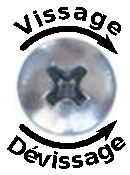
\includegraphics[width=\tailleImageTournevis]{pics/sens-vissage.pdf}
\begin{minipage}[][][c]{0.12\columnwidth}
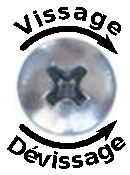
\includegraphics[width=\columnwidth]{pics/sens-vissage.pdf}
%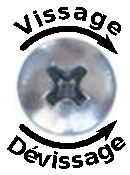
\includegraphics[width=\formCoefficient*\columnwidth]{pics/sens-vissage.pdf}
\end{minipage}

%TODO http://tex.stackexchange.com/questions/30081/how-can-i-sum-two-values-and-store-the-result-in-other-variable/30083#30083

\textbf{Différents tournevis~:} Il existe différentes formes et tailles de tournevis, utiliser la plus adaptée permet de préserver l'empreinte de la vis ainsi que de protéger l'extrémité de l'outil.

\begin{center}
%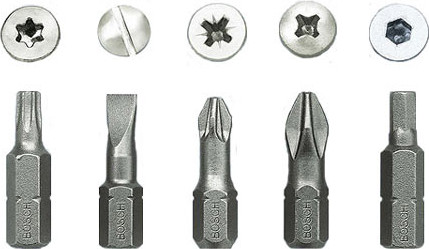
\includegraphics[width=\tailleImageTournevis]{pics/types-tournevis.jpg}
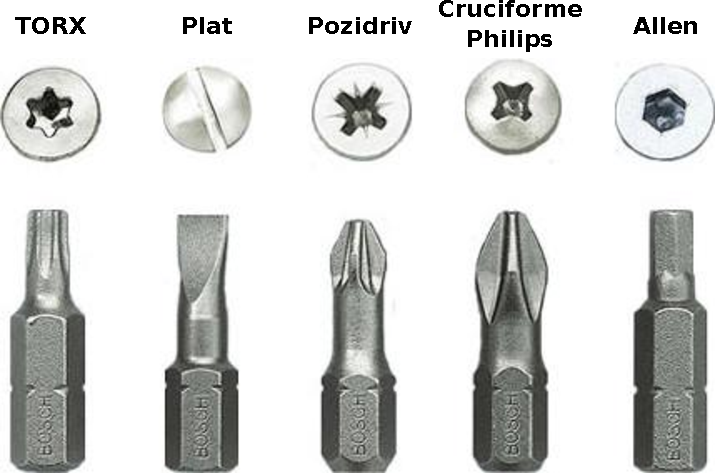
\includegraphics[width=\tailleImageTournevis]{pics/types-tournevis.pdf}
%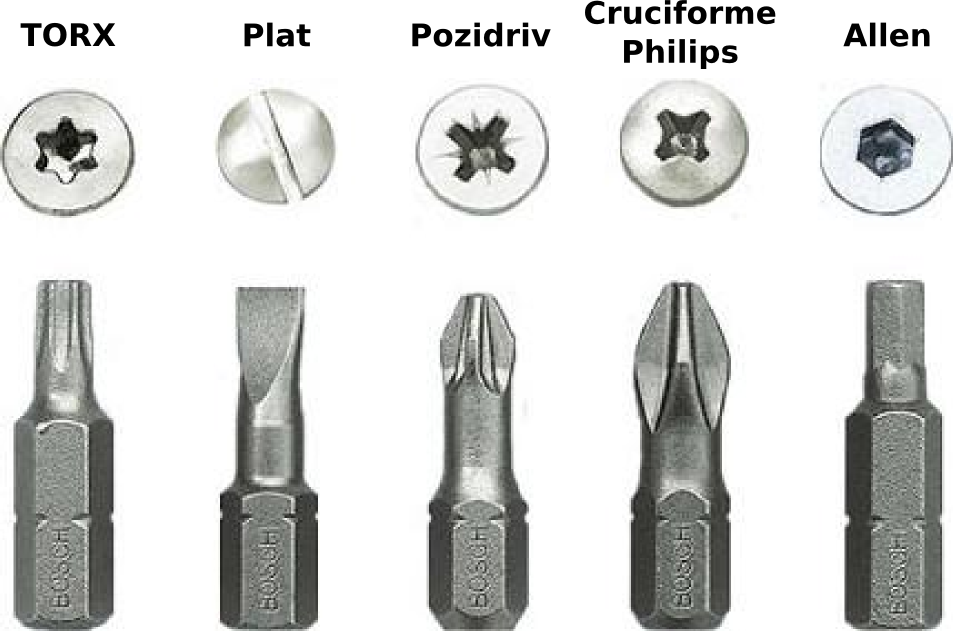
\includegraphics[width=\tailleImageTournevis]{pics/types-tournevis.png}
\end{center}

\textbf{Les clefs~:}  Elles servent à serrer et desserrer les vis, les boulons, et les écrous. Adaptez la dimension de la mâchoire de votre clef à la dimension de l'objet que vous devez, en vous aidant de la molette de la clef, il ne reste plus qu'à visser. \todo{Parler aussi des clefs à pipes, clefs plate, ...}

\textbf{Types de vis~:} pour différents matériaux à utiliser avec le bon tournevis.

\begin{center}
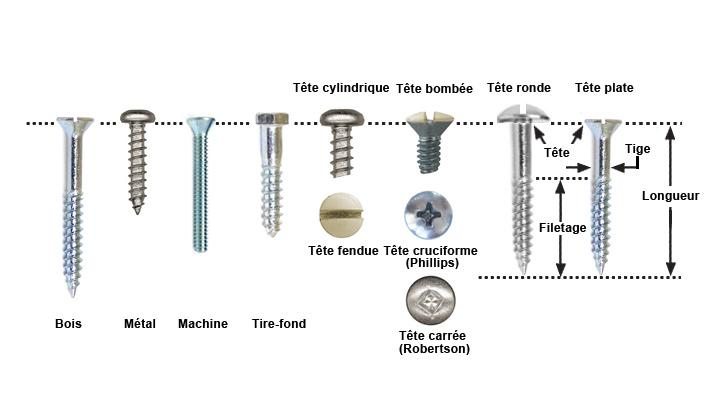
\includegraphics[width=\tailleImageTournevis]{pics/types-vis.jpg}
\end{center}
